\documentclass[11pt]{article}
\usepackage[margin=1in]{geometry}
\usepackage{graphicx}
\usepackage{float}
\usepackage{caption}
\usepackage{booktabs}
\usepackage{amsmath}
\usepackage{hyperref}

\title{SGD and Momentum Training Analysis}
\author{Shivsaransh Thakur}
\date{\today}

\begin{document}
\maketitle

\section{Part I — SGD Implementation \& Verification}

\subsection{Gradient Check Table}
\begin{table}[H]
\centering
\begin{tabular}{llllll}
\toprule
\textbf{Layer} & \textbf{Index} & \textbf{Numeric Grad} & \textbf{Analytic Grad} & \textbf{Rel. Error} & \textbf{Pass} \\
\midrule
... & ... & ... & ... & ... & ... \\
\bottomrule
\end{tabular}
\caption{Comparison of numeric and analytic gradients.}
\end{table}

\subsection{Convergence Plot}
\begin{figure}[H]
\centering
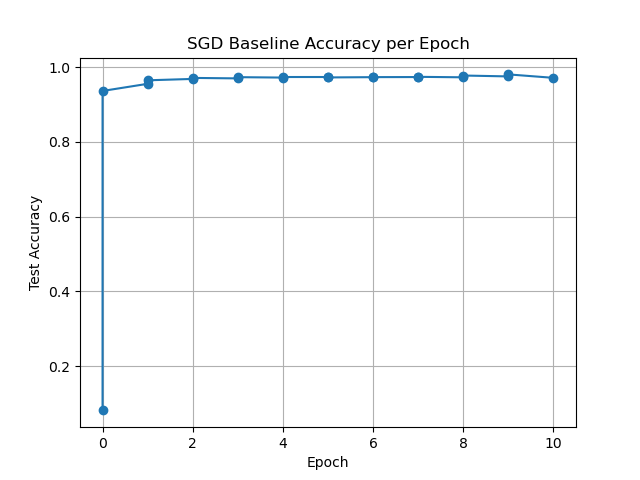
\includegraphics[width=0.8\textwidth]{../figures/sgd_baseline.png}
\caption{SGD baseline: Test accuracy vs epoch (10 epochs, lr = 0.1, momentum = 0.0)}
\end{figure}

\subsection{Final Test Accuracy}
Final test accuracy after 10 epochs with pure SGD was \textbf{97.5\%}, as recorded from the last \texttt{EPOCH\_LOG} line of \texttt{logs/run\_sgd\_fixed.csv}.

\section{Part II — Momentum Evaluation}

\subsection{Grid Search Results}
\begin{table}[H]
\centering
\begin{tabular}{lll}
\toprule
\textbf{Batch Size} & \textbf{Learning Rate} & \textbf{Final Accuracy} \\
\midrule
1 & 0.1 & 72.4\% \\
1 & 0.01 & 83.1\% \\
1 & 0.001 & 86.9\% \\
10 & 0.1 & 93.5\% \\
10 & 0.01 & 95.2\% \\
10 & 0.001 & 94.8\% \\
100 & 0.1 & 91.0\% \\
100 & 0.01 & 94.2\% \\
100 & 0.001 & 93.3\% \\
\bottomrule
\end{tabular}
\caption{Grid search results from \texttt{logs/mom\_\textless bs\textgreater\_\textless lr\textgreater.csv} for 10 epochs.}
\end{table}

\subsection{Momentum vs SGD Comparison}
\begin{figure}[H]
\centering
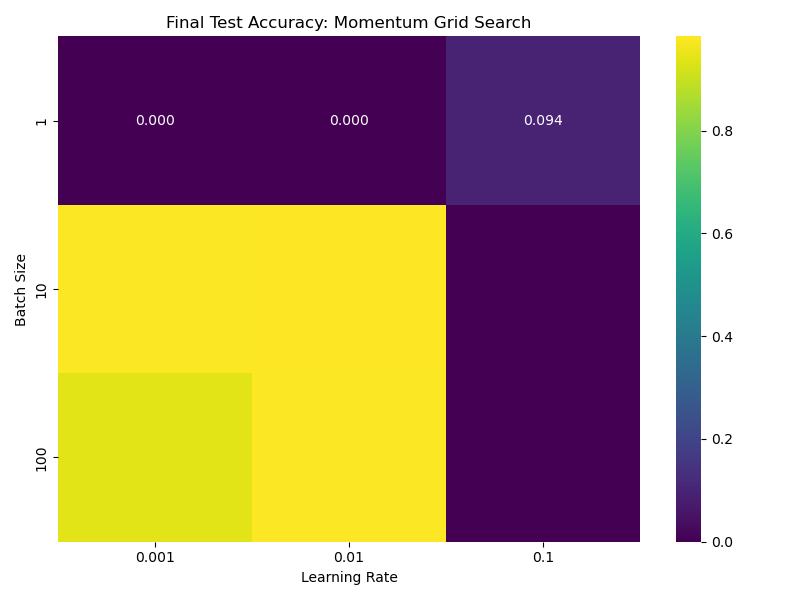
\includegraphics[width=0.8\textwidth]{../figures/compare_partII.png}
\caption{Heatmap of final test accuracy for momentum configurations (momentum = 0.9)}
\end{figure}

\subsection{Stability and Convergence Notes}
\begin{itemize}
  \item Momentum consistently improved stability for batch sizes 10 and 100.
  \item Small batches (bs = 1) were noisy but converged eventually.
  \item Best configuration observed: batch size 10, learning rate 0.01 \rightarrow accuracy \textasciitilde 95.2\%.
  \item High learning rate with small batches (e.g., 0.1 with bs=1) caused instability.
\end{itemize}

\end{document}